\chapter{Revisão da Literatura}
Neste capítulo, são abordados os principais conceitos usados para o entendimento do projeto Turma de Elite.

\section{\textit{Learning Management System (LMS)}}
Os \textit{\ac{lms}} – são plataformas de apoio à aprendizagem e surgiram para atender as necessidades da formação à distância online. Essas plataformas facilitam a disponibilização de recursos em diferentes formatos como texto, vídeo e áudio, apontadores para sites, avisos, interação professor-alunos através de ferramentas de comunicação, ferramentas de apoio à aprendizagem colaborativa e registro das atividades realizadas pelos alunos \cite{rentabilizacao-ens-basico-e-secundario:2007}.

Elas possuem diversas vantagens como agilidade, escalabilidade, engajamento dos alunos, integração e acessibilidade. Estas vantagens faz com que essas plataformas sejam atrativas, considerando ainda, o cenário atual de globalização, onde há a vasta utilização da internet para diversas atividades, inclusive para os estudos.

%A pandemia de 2020 também foi um fator que causou mudanças no modo como vivemos e realizamos nossas atividades cotidianas. Ainda segundo o Censo da Educação Superior, o EAD é a modalidade que mais cresce no Brasil e já possui 21,2\% do total de matrícula do ensino superior, além disso, esse formato de aprendizagem proporciona flexibilidade de horários e democratiza e educação, visto que, diversas universidades disponibilizam gratuitamente custos online \cite{ead-ces}.


\section{\textit{Gamificação}}
Um \textit{game} pode ser definido por meio de regras, interatividade e \textit{\gls{feedback}}, gerando assim um resultado quantificável, muitas vezes provocando uma reação emocional. Em um contexto envolvendo \textit{games} e aprendizagem, \cite{gamification-of-learning:2012} adiciona o conceito de relação emocional, baseada em uma ideia de diversão proporcionada por esta junção de elementos \cite{gamification-of-learning:2012}.
A \textit{gamificação}, por sua vez, é uma técnica que envolve dinâmicas, mecanismos e elementos dos \textit{videogames}, como objetivos, obstáculos e competitividade, e os aplica em contextos da vida real, ou simplesmente que não sejam necessariamente de um jogo. O principal objetivo é engajar as pessoas para que mudem alguns comportamentos, com o propósito de alcançar resultados relacionados a objetivos específicos \cite{gamificação-na-ead:2014}.


A \textit{gamificação} surge justamente para auxiliar nessa demanda. Em situações em que o engajamento é precário, é possível estabelecer um estímulo extra em contextos que nada têm a ver com jogos, como ambientes corporativos e educacionais
\cite{gamificacao-corporativa:2017}.


Desse modo, pode-se afirmar que a \textit{gamificação} é um processo dedicado ao engajamento de pessoas para que elas produzam mais, independentemente do setor em que estejam inseridas. Seu objetivo é justamente oferecer uma maior motivação para que as pessoas possam se divertir ao realizar tarefas que elas já precisariam fazer de uma forma ou de outra. \cite{gamificacao-corporativa:2017}

\section{Recompensa}
A recompensa se refere a um prêmio ou retribuição por algo \cite{dicio-recompensa:2009}.


Todos gostam de se sentir valorizados por aquilo que produzem. Assim é importante que os gestores se lembrem de implementar alguns mecanismos de recompensas que motivem os colaboradores \cite{gamificacao-corporativa:2017}. Por isso que, no contexto escolar, essa valorização é de suma importância para que estudantes possam ter a segurança de que estão fazendo a coisa certa, e poderão ser incentivados a continuar a realizar um bom trabalho.

Existem inúmeras formas de recompensar um usuário através da \textit{gamificação}, como por exemplo sistemas de pontuação, medalhas, objetos colecionáveis, ou simplesmente o recebimento de reconhecimento. Elas podem ser concebidas de maneira pré-estabelecida ao realizar-se determinado desafio ou de maneira imprevista.


Constata-se que a maioria dos indivíduos associam a motivação com o reconhecimento por performance \cite{grafico-motivacao:2012}. A \autoref{fig:recompensa} demonstra que tal reconhecimento é o fator preponderante na geração de motivação nas pessoas para a execução de atividades.

\begin{figure}[htb]
    \centering
	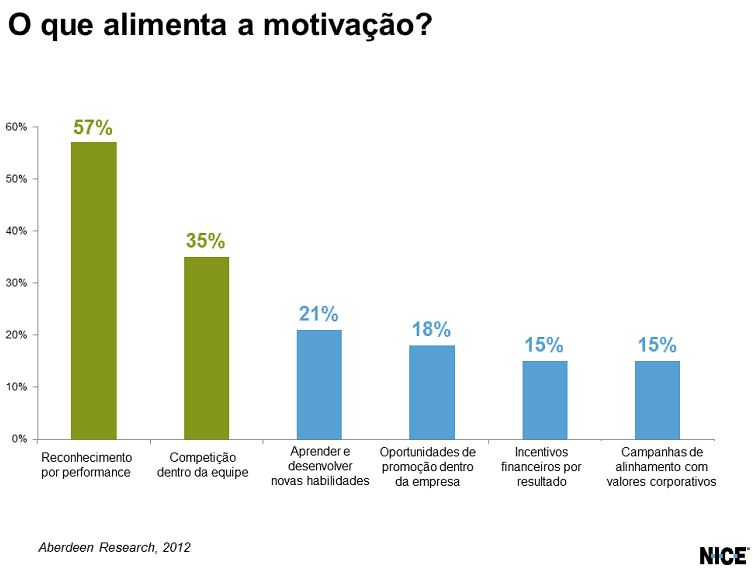
\includegraphics[width=16cm]{imagens/recompensa.jpg}
	\caption{\label{fig:recompensa}O que alimenta a motivação?}
	\fonte{\cite{grafico-motivacao:2012}}
\end{figure}
\FloatBarrier

Além do reconhecimento ser uma grande solução para motivar um indivíduo, pode-se ver na \autoref{fig:recompensa} que outro método bastante efetivo é através da competitividade. Esta por sua vez, não tem a necessidade de ser estimulada diretamente, como ao promover um vencedor em um jogo. O fato de simplesmente parabenizar as melhores notas de uma turma em uma prova ou atividade, por exemplo, já é o suficiente para gerar um certo nível de competição de forma saudável. Fora o fato de que competições, quando são realizadas em grupos, podem ser importantes fatores para reforçar o trabalho em equipe \cite{gamificação-na-ead:2014}.


